% Build with build.bat (XeLaTeX, Biber, XeLaTeX, XeLaTeX).
\documentclass[10pt,a4paper]{article}
\usepackage{twente-paper}
\addbibresource{references.bib}
% Use \gls{key}, \Gls{key}, or \glspl{key} in the manuscript.
% Used entries appear automatically and terms link to their definitions.
\newglossaryentry{synthetic-data}{name={synthetic data},
  description={Artificially generated data designed to represent selected properties of observed or target data}}
% Abbreviations are displayed as short forms; the full name is in the glossary.
\newglossaryentry{machine-learning}{name={ML},
  description={Machine learning: methods that learn patterns from data to perform tasks such as prediction or classification}}
\newglossaryentry{gan}{name={GAN},plural={GANs},
  description={Generative adversarial network: a generative modelling approach in which a generator and a discriminator are trained with competing objectives}}
\newglossaryentry{ctgan}{name={CTGAN},
  description={Conditional tabular generative adversarial network: a GAN-based approach to generating synthetic tabular data using conditional generation}}
\newglossaryentry{fidelity}{name={fidelity},
  description={The extent to which synthetic data reproduce relevant properties of the target data}}
\newglossaryentry{utility}{name={utility},
  description={The usefulness of data for a specified downstream task and evaluation setting}}
\newglossaryentry{lidar}{name={LiDAR},
  description={Light detection and ranging: a sensing technique that uses laser light to measure distances to surfaces; scanning systems combine these measurements into a point cloud}}
\newglossaryentry{point-cloud}{name={point cloud},plural={point clouds},
  description={A collection of points in three-dimensional space, often with additional attributes such as return intensity; a sensor scan usually observes only part of a scene}}
\newglossaryentry{range-image}{name={range image},plural={range images},
  description={An image-like representation in which each pixel stores a measured distance for a viewing direction, such as a LiDAR beam direction}}
\newglossaryentry{intensity}{name={intensity},
  description={A sensor-reported measure of the strength of a returned LiDAR signal; its value depends on the surface, measurement geometry and sensor processing}}
\newglossaryentry{ray-casting}{name={ray casting},
  description={Computing intersections of simulated rays with scene geometry, for example to determine distances along LiDAR beam directions}}
\newglossaryentry{ray-drop}{name={ray drop},
  description={The absence of a recorded return for a LiDAR beam, for example because too little reflected light reaches the receiver}}
\newglossaryentry{surfel}{name={surfel},plural={surfels},
  description={Surface element: a small local surface patch, often represented by an oriented disk, used to approximate scene or object geometry}}
\newglossaryentry{occlusion}{name={occlusion},
  description={A nearer object or surface blocking a sensor's view of another part of a scene}}
\newglossaryentry{object-detection}{name={3D object detection},
  description={Identifying object categories and locating objects in three-dimensional space, commonly using oriented bounding boxes}}
\newglossaryentry{semantic-segmentation}{name={semantic segmentation},
  description={Assigning a semantic class, such as road or vehicle, to each pixel or point in an observation}}
\newglossaryentry{domain-gap}{name={domain gap},
  description={Differences between source and target data distributions, such as simulated and real sensor data, that can affect model transfer}}
\newglossaryentry{domain-randomization}{name={domain randomization},
  description={Varying generation or simulation parameters to expose a training model to a range of conditions and investigate transfer beyond a single simulated setting}}
\newglossaryentry{procedural-generation}{name={procedural generation},
  description={Constructing data or scene content through rules, algorithms and parameters rather than specifying every output individually}}
\newglossaryentry{augmentation}{name={data augmentation},
  description={Creating training variants by transforming or combining available examples, while maintaining or updating their labels as required}}
\newglossaryentry{bayesian-network}{name={Bayesian network},plural={Bayesian networks},
  description={A probabilistic model that represents variables and their conditional dependencies using a directed acyclic graph}}
\newglossaryentry{vae}{name={VAE},plural={VAEs},
  description={Variational autoencoder: a probabilistic generative model with a latent representation, a decoder and an encoder that approximates inference over the latent variables}}
\newglossaryentry{tvae}{name={TVAE},
  description={Tabular variational autoencoder: a VAE adapted to generating tabular records}}
\newglossaryentry{diffusion-model}{name={diffusion model},plural={diffusion models},
  description={A generative model trained to reverse a gradual corruption process, commonly producing samples through successive denoising steps}}
\newglossaryentry{score-function}{name={score function},
  description={In score-based generation, the gradient of the log probability density with respect to the data; a learned estimate guides sampling towards regions of higher probability}}
\newglossaryentry{langevin-dynamics}{name={annealed Langevin dynamics},
  description={An iterative sampling procedure combining score-guided updates with random noise across a sequence of decreasing noise levels}}
\newglossaryentry{normalizing-flow}{name={normalizing flow},plural={normalizing flows},
  description={A generative model that transforms a simple reference distribution through invertible mappings}}
\newglossaryentry{mode-collapse}{name={mode collapse},
  description={A failure of a generative model to represent parts of the target distribution, producing insufficiently varied samples}}
\newglossaryentry{fid}{name={FID},
  description={Fr\'echet Inception Distance: a comparison of Gaussian approximations to feature distributions from real and generated images; the feature representation matters and suitability for LiDAR is not automatic}}
\newglossaryentry{ap}{name={AP},
  description={Average precision: a summary of a precision--recall curve; object-detection results depend on the matching rules, thresholds and benchmark protocol}}
\newglossaryentry{miou}{name={mIoU},
  description={Mean intersection over union: the average across evaluated classes of the overlap between predicted and reference segments divided by their union}}

% Canonical wording used by the paper, proposal and Beamer slides.
% RQ1--RQ3 are subquestions of the main research question.
\newcommand{\MainResearchQuestion}{How can synthetic data generation methods support the creation of LiDAR point clouds for training perception models in autonomous driving?}
\newcommand{\GenerationQuestion}{What are the main approaches to generating synthetic data for machine learning, and what are their assumptions and trade-offs?}
\newcommand{\LidarQuestion}{How are these approaches applied to generate LiDAR point clouds, and how do they address sensor realism, scene diversity and annotation needs?}
\newcommand{\EvaluationQuestion}{How are synthetic LiDAR datasets evaluated, and which metrics best indicate their usefulness for training neural networks that perform on real-world data?}

% Topic contact confirmed by the authors; public details verified on UT's
% official profile: https://people.utwente.nl/g.a.folkertsma
\newcommand{\TopicContactName}{dr.ir. G.A. Folkertsma (Geert)}
\newcommand{\TopicContactEmail}{g.a.folkertsma@utwente.nl}
\newcommand{\TopicContactProfile}{https://people.utwente.nl/g.a.folkertsma}
\newcommand{\TopicContactLink}{\href{\TopicContactProfile}{\TopicContactName}}
% EE/ROB topics contact supplied by the authors; no email or title assumed.
\newcommand{\EEROBContactName}{dr.ir. J.T.W. Berendsen (Jorien)}
\newcommand{\EEROBContactEmail}{j.t.w.berendsen@utwente.nl}
\newcommand{\EEROBContactProfile}{https://people.utwente.nl/j.t.w.berendsen}
\newcommand{\EEROBContactLink}{\href{\EEROBContactProfile}{\EEROBContactName}}
% Student addresses supplied by the authors (not inferred from their names).
\newcommand{\LaporteEmail}{f.p.s.laporte@student.utwente.nl}
\newcommand{\KeglerEmail}{o.c.f.kegler@student.utwente.nl}
\newcommand{\LaporteEmailLink}{\href{mailto:\LaporteEmail}{\LaporteEmail}}
\newcommand{\KeglerEmailLink}{\href{mailto:\KeglerEmail}{\KeglerEmail}}
\newcommand{\TopicContactEmailLink}{\href{mailto:\TopicContactEmail}{\TopicContactEmail}}
\newcommand{\EEROBContactEmailLink}{\href{mailto:\EEROBContactEmail}{\EEROBContactEmail}}
% General campus visiting address, not the contact person's office address.
% Source: https://www.utwente.nl/en/about-us/campus/contact-route/
\newcommand{\UTStreet}{Drienerlolaan 5}
\newcommand{\UTCityCountry}{7522 NB Enschede, The Netherlands}
\newcommand{\UTAddress}{\UTStreet, \UTCityCountry}

\hypersetup{pdftitle={Synthetic Data Generation: From General Methods to LiDAR Perception},pdfauthor={Frans Laporte and Florent Kegler}}
\begin{document}
% Avoid duplicate PDF page destinations on the two unnumbered title pages.
\hypersetup{pageanchor=false}
\begin{titlepage}
\thispagestyle{empty}
\begin{tikzpicture}[remember picture,overlay,x=1mm,y=1mm]
  \fill[ink] (current page.north west) rectangle ([yshift=-210mm]current page.north east);
  \begin{scope}[shift={(current page.north west)}]
    \node[anchor=north west,text=white,inner sep=0] at (24,-22) {\fontsize{8}{10}\selectfont\bfseries ACADEMIC RESEARCH SKILLS};
    \node[anchor=north east,text=white,inner sep=0] at (186,-22) {\fontsize{8}{10}\selectfont OCTOBER 2026};
    \draw[white,line width=.35pt] (24,-32)--(186,-32);
    \node[anchor=north west,text=white,inner sep=0] at (24,-43) {\fontsize{9}{11}\selectfont LITERATURE REVIEW};
    \node[anchor=north west,text=white,text width=166mm,inner sep=0] at (23,-58) {\fontsize{38}{40}\selectfont\bfseries Synthetic LiDAR \\Point Cloud Generation\par};
    \node[anchor=north west,text=white,text width=150mm,inner sep=0] at (24,-94) {\fontsize{18}{23}\selectfont Methods and Evaluation\\ for Autonomous Driving\par};
    % Original artwork: irregular observations become a synthetic grid.
    \begin{scope}
      \clip (24,-130) rectangle (186,-196);
      \foreach \i in {0,...,23}{
        \pgfmathsetmacro{\ya}{-137-\i*2.15}
        \pgfmathsetmacro{\yb}{\ya+5*sin(\i*37)}
        \draw[white,opacity=.22,line width=.35pt] (24,\yb) .. controls (79,\yb+16) and (117,\ya-16) .. (186,\ya);
      }
      \foreach \i in {0,...,9}{\foreach \j in {0,...,6}{
        \pgfmathsetmacro{\xx}{27+\i*4.1+1.4*sin(\i*67+\j*39)}
        \pgfmathsetmacro{\yy}{-143-\j*7+2*cos(\i*41+\j*61)}
        \fill[white,opacity=.8] (\xx,\yy) circle (.48);
      }}
      \foreach \i in {0,...,9}{\foreach \j in {0,...,6}{
        \draw[white,opacity=.85,line width=.45pt] (142+\i*4.6,-140-\j*7) circle (.65);
      }}
      \draw[white,line width=.8pt] (105,-166) circle (14);
      \draw[white,line width=.7pt,-{Stealth[length=2mm]}] (97,-166)--(113,-166);
    \end{scope}
    \node[anchor=west,text=white,inner sep=0] at (24,-202) {\fontsize{6.5}{8}\selectfont OBSERVATIONS};
    \node[anchor=center,text=white,inner sep=0] at (105,-202) {\fontsize{6.5}{8}\selectfont REPRESENTATION};
    \node[anchor=east,text=white,inner sep=0] at (186,-202) {\fontsize{6.5}{8}\selectfont SYNTHETIC SAMPLES};
    % Full author details, contacts and address are on the formal title page.
    % Aligned labels and a shared rule make the lower area one coherent block.
    \draw[rulegray,line width=.5pt] (24,-232)--(186,-232);
    \node[anchor=north west,inner sep=0,text=muted] at (24,-239) {\fontsize{8}{10}\selectfont\bfseries AUTHORS};
    \node[anchor=north west,inner sep=0] at (24,-249) {\fontsize{14}{18}\selectfont Frans Laporte};
    \node[anchor=north west,inner sep=0] at (24,-260) {\fontsize{14}{18}\selectfont Florent Kegler};
    \node[anchor=north west,inner sep=0,text=muted] at (136,-239) {\fontsize{8}{10}\selectfont\bfseries INSTITUTION};
    % Official image supplied in Images; retain its original aspect ratio.
    \node[anchor=north east,inner sep=0] at (186,-249) {
\includegraphics[width=50mm]{Images/UTLogo.png}};
  \end{scope}
\end{tikzpicture}
\null
\end{titlepage}


% Formal title page after the illustrated cover; neither displays a page number.
\begin{titlepage}
\thispagestyle{empty}
\eyebrow{University of Twente / Academic Research Skills}
\vspace{6mm}
{\fontsize{30}{34}\selectfont\bfseries Synthetic LiDAR Point Cloud \\Generation\par}
\vspace{4mm}
{\fontsize{18}{23}\selectfont Methods and Evaluation for Autonomous Driving\par}
\vspace{3mm}
{\color{muted}Literature review\par}
\vspace{4mm}
{\color{rulegray}\hrule}
\vspace{4mm}

\begin{minipage}[t]{.48\linewidth}
\eyebrow{Student authors}
\vspace{3mm}
Frans Laporte BSc.\par
\LaporteEmailLink\par
\vspace{3mm}
Florent Kegler BSc.\par
\KeglerEmailLink
\end{minipage}\hfill
\begin{minipage}[t]{.48\linewidth}
\eyebrow{Topic contact}
\vspace{3mm}
\TopicContactLink\par
\TopicContactEmailLink\par
\vspace{3mm}
\eyebrow{EE/ROB topics contact}
\vspace{3mm}
\EEROBContactLink\par
\EEROBContactEmailLink
\end{minipage}

\vspace{6mm}
\eyebrow{Course and institutional context}
\vspace{3mm}
Academic Research Skills\par
Faculty of Electrical Engineering, Mathematics and Computer Science\par
University of Twente

\vspace{4mm}
\eyebrow{Place and date}
\vspace{3mm}
Enschede, \today

\vspace{4mm}
\eyebrow{Acknowledgement of AI assistance}
\vspace{2mm}
{\small\color{muted}OpenAI ChatGPT was used to rephrase text, review the structure of the document, and help identify academic sources.
The authors remain responsible for verifying sources, assessing the evidence
and approving the final text.\par}

\vfill
{\color{rulegray}\hrule}
\vspace{3mm}
\begin{minipage}[c]{.62\linewidth}
{\small\color{muted}University of Twente\par
\UTStreet\par
\UTCityCountry}
\end{minipage}\hfill
\begin{minipage}[c]{.32\linewidth}

\includegraphics[width=\linewidth]{Images/UTLogo.png}
\end{minipage}
\end{titlepage}

\pagenumbering{roman}
\hypersetup{pageanchor=true}
\eyebrow{Literature review / Research overview}
% \section*{At a glance} got a question mark in the review so comment out
\vspace{3mm}
\begin{researchbox}{Abstract}
Synthetic data offers a means of expanding training datasets for automotive LiDAR perception while providing control over scene composition and annotations. However, differences between generated scans and real measurements can limit the transfer of trained perception models, making the usefulness of synthetic data generation approaches with their application to automotive LiDAR object detection and semantic segmentation. Statistical models, procedural simulation, learned generators and hybrid approaches are examined in terms of scene control, coverage, annotation support and dependence on data observed in the real world. The review then considers how sensor sampling, occlusion, missing returns and intensity influence the generated observations, before assessing the evidence provided by similarity metrics and downstream perception experiments. The selected studies demonstrate benefits in particular training settings, but differences in datasets, tasks and evaluation protocols prevent a general ranking of generation methods. Their findings indicate that geometric or distributional similarity alone is not enough to accomplish training utility, which requires evaluation on independent real data under roughly the same conditions. Synthetic LiDAR therefore has demonstrated value as a targeted supplement to real world training data, while the relationship between sensor fidelity, scenario coverage and downstream performance remains an area for further investigation.
\end{researchbox}

\vspace{5mm}
\eyebrow{Keywords}
Synthetic data\quad /\quad Machine learning\quad /\quad Data quality\quad /\quad Literature review
\vspace{11mm}
% \tableofcontents was not needed in the review so comment out
\clearpage
\pagenumbering{arabic}
\section{Introduction}
\label{sec:introduction}

Autonomous-driving perception requires an understanding of the objects
and surfaces surrounding a vehicle. \Gls{lidar} provides
three-dimensional measurements of the environment that support tasks
such as \gls{object-detection} and \gls{semantic-segmentation}
\parencite{geigerAreWeReady2012a,behleySemanticKITTIDatasetSemantic2019}.
Developing learning-based methods for these tasks requires annotated
data, but collecting and labelling automotive \glspl{point-cloud} is
intensive. Furthermore, uncommon traffic situations are difficult
to capture in sufficient numbers through ordinary data collection.
These constraints motivate the generation of \gls{synthetic-data},
which offers opportunities to produce annotated observations and
construct controlled scenarios
\parencite{hurlPreciseSyntheticImage2019,
	manivasagamLiDARsimRealisticLiDAR2020,xiaoTransferLearningSynthetic2022}.

The potential of synthetic data depends on how the data is
generated. Virtual environments can provide scene control and automatic
annotations, as demonstrated by PreSIL and SynLiDAR
\parencite{hurlPreciseSyntheticImage2019,
	xiaoTransferLearningSynthetic2022}.
Other approaches draw more directly on real observations. LiDARsim
combines reconstructed scenes with physical simulation and a learned
model of missing returns, while LiDARGen learns to generate scans from
examples
\parencite{manivasagamLiDARsimRealisticLiDAR2020,
	zyrianovLearningGenerateRealistic2022}.
Together, these approaches show different balances between
explicit control over the scene and dependence on data observed in the real world.
Understanding these differences provides a basis for assessing which
generation approaches can meet the requirements of a particular
perception task.

For automotive LiDAR, those requirements extend beyond the geometry of
the scene. A scan samples visible surfaces from a particular viewpoint,
and its structure depends on sensor sampling, \gls{occlusion} and
missing returns. LiDARsim illustrates the importance of modelling this
observation process, while SynLiDAR identifies differences in appearance
and sparsity as components of the \gls{domain-gap} between synthetic
and real point clouds
\parencite{manivasagamLiDARsimRealisticLiDAR2020,
	xiaoTransferLearningSynthetic2022}.
Consequently, the assessment of synthetic data must connect the
properties of generated scans with their intended use. LiDARGen
evaluates scan generation and completion, whereas PreSIL and SynLiDAR
also investigate the contribution of synthetic data to training
perception models
\parencite{zyrianovLearningGenerateRealistic2022,
	hurlPreciseSyntheticImage2019,xiaoTransferLearningSynthetic2022}.
These evaluations provide different forms of evidence, making it
necessary to distinguish similarity to real world observations from
demonstrated benefits for learning on real world data.

This narrative review examines that connection through selected
literature on synthetic-data generation and its application to
scene level automotive LiDAR perception. General generation approaches
provide the conceptual foundation, while LiDAR-specific studies form
the basis for discussing object detection and semantic segmentation.
The scope includes virtual-scene simulation, reconstruction-based
simulation and learned scan generation. Scan completion is considered
where it clarifies the capabilities of a method, while its results are
distinguished from evidence obtained by training with newly generated
data. This scope supports a comparison of generation capabilities,
sensor-specific requirements and evaluation practices without assuming
that results from different tasks and datasets are directly comparable.

The review first examines the principal generation approaches and
their implications for control, coverage and dependence on real data.
It then considers their application to automotive LiDAR, focusing on
scene construction, sensor modelling and annotation consistency.
These requirements provide the basis for examining evaluation metrics
and evidence of transfer to real perception tasks. The discussion
subsequently brings these findings together to identify limitations
and directions for further investigation. The review therefore begins
with the generation approaches that underpin the construction and
assessment of synthetic LiDAR data.

\section{Background and terminology}
\label{sec:background}
Simulation models how a scene produces an observation; learned generation
estimates a sampling process from examples; \gls{augmentation} transforms
or recombines existing data. These categories overlap, and synthetic-only
perception training can still depend on real assets or generator training
data \parencite{nikolenkoSyntheticDataDeep2019,manivasagamLiDARsimRealisticLiDAR2020a}.

A LiDAR scan samples visible surfaces rather than complete geometry.
Beam directions, \gls{occlusion}, \gls{intensity}, missing returns and
motion shape the observation. Point sets, \glspl{range-image} and
\glspl{voxel} expose different spatial structure; representation and
sensor assumptions must accompany a generation claim
\parencite{zyrianovLearningGenerateRealistic2022,manivasagamZeroDomainGap2023}.

Realism, coverage and downstream \gls{utility} are distinct.
\Textcite{alaaHowFaithfulYour2022} distinguish fidelity, diversity and
generalization, with Authenticity addressing copying of training data.
The tabular evaluation survey by \textcite{achterbergMetricsThatMatter2026},
available as a preprint, likewise makes metric choice depend on task and
context. These frameworks motivate multiple assessment dimensions; they do
not establish a LiDAR-specific proxy for real perception performance.

\eyebrow{Approach / From search to synthesis}
\section{Review methodology}
\label{sec:methodology}

This focused narrative review uses the shared Zotero collection, targeted
source checks on 1 October 2026, and follow-up full-text checks on
5 October 2026, supplemented by targeted numerical and publication-record
checks on 27 October 2026. The selected sources support the synthesis: general surveys and
methodological studies provide context, while LiDAR generation, transfer
and benchmark papers provide sensor-specific evidence. Follow-up retrieval
used exact-title searches and publisher or author records. Query histories,
claim locations and numerical checks are retained in the research notes.


The selection is illustrative rather than exhaustive: complete database
exports and screening totals were not recorded. Targeted source checks
include AI-assisted extraction, with the checking method documented in the
research notes; no independent duplicate-screening record is available.
Preprints are identified, duplicate
versions are not counted separately, and tabular or language-model findings
are not treated as direct LiDAR evidence.


We compare generation task, representation, real-data requirements,
annotations and evaluation setting. Results remain separate when class
sets, sensors, models or training regimes differ: BEV detection is not full
3D detection, and scan completion is not synthetic-data training. No new
experiments, pooled effects or statistical significance claims are made.


\section{Synthetic data generation approaches}
\label{sec:rq1}

Synthetic data generation methods differ in how they represent the process
that produces an observation. Statistical and learned models infer
relationships from examples, whereas simulation explicitly describes
scenes and their observation. Hybrid approaches combine these strategies.
This review uses these four groups to organise the literature, rather than
as mutually exclusive categories. They provide a basis for comparing how
generation methods control the resulting data, represent variation and
depend on real observations
\parencite{hernandezSyntheticDataGeneration2022,
nikolenkoSyntheticDataDeep2019,manivasagamLiDARsimRealisticLiDAR2020}.
Related \gls{augmentation} techniques transform or recombine existing
examples, so their contribution depends on both the original data and
whether the transformations preserve the required labels
\parencite{nikolenkoSyntheticDataDeep2019}.

\subsection{Statistical models}

Statistical generators produce samples from fitted distributions that
describe relationships between variables. For example,
\glspl{bayesian-network} represent conditional dependencies, allowing new
records to be sampled from the fitted model. The review by Hernandez et al.
and the benchmark by Hansen et al. discuss such methods for tabular data,
where observations consist of numerical or categorical attributes
\parencite{hernandezSyntheticDataGeneration2022,
hansenReimaginingSyntheticTabular2023}.
These studies establish a general approach to modelling data dependencies,
but do not demonstrate that tabular generators reproduce the spatial
structure of automotive LiDAR scans. Their relevance here is the underlying
principle that generated samples reflect the relationships represented by
the model. Increasing the number of samples cannot by itself recover
relationships that were omitted or poorly estimated, and uncertainty in
the fitted generator therefore remains relevant when synthetic datasets
are enlarged \parencite{breugelSyntheticDataReal2023}.

\subsection{Procedural and physical simulation}

Simulation provides a different form of control by specifying how scenes
are constructed and how a sensor observes them. Procedural rules define
scene content and variation, while the observation model converts that
content into measurements. This separation allows scene configurations to
be varied deliberately and annotations to be derived from known scene
properties. However, the generated observations remain constrained by the
available assets and the effects represented in the simulator
\parencite{nikolenkoSyntheticDataDeep2019,
manivasagamLiDARsimRealisticLiDAR2020}.
\Gls{domain-randomization} broadens the generated conditions by varying
selected parameters. Its usefulness consequently depends on which
parameters are varied and how their values are sampled, rather than on
variation alone \parencite{nikolenkoSyntheticDataDeep2019}.
For LiDAR perception, this distinction motivates examining scene diversity
and sensor modelling separately: changing the objects in a scene does not
necessarily correct how the simulated sensor samples their surfaces.

\subsection{Learned generators}

Learned generators model patterns in example data without requiring every
relationship to be specified explicitly. Approaches include
\glspl{vae}, which generate through a learned latent representation,
\glspl{gan}, which use adversarial training, and
\glspl{diffusion-model}, which learn a denoising process.
Hansen et al. compare representatives of these families in a tabular
setting, illustrating the range of available modelling approaches rather
than establishing a preferred method for LiDAR
\parencite{hansenReimaginingSyntheticTabular2023}.
Their flexibility also makes the training examples important: plausible
individual samples do not establish that a generator covers the full
distribution, and effects such as \gls{mode-collapse} can restrict the
variation represented \parencite{breugelSyntheticDataReal2023}.

LiDARGen provides a sensor-specific example of learned generation. It
represents scans as range and intensity images, learns through
\gls{score-matching}, and generates samples using iterative
\gls{langevin-dynamics}. It also supports conditional scan densification
\parencite{zyrianovLearningGenerateRealistic2022}.
This demonstrates how a learned model can represent scan structure, but
does not make scan generation equivalent to constructing an annotated
training dataset. Semantic labels and explicit control of scene objects
are additional requirements that cannot be inferred from plausible range
and intensity values alone. Learned generation must therefore be assessed
against the intended use of its outputs, including the annotations and
controls needed by the perception task.

\subsection{Hybrid approaches and implications for LiDAR}

Hybrid pipelines retain explicit scene or sensor structure while learning
components that are difficult to describe analytically. LiDARsim combines
assets reconstructed from real recordings with \gls{ray-casting} and a
learned \gls{ray-drop} model. The geometric model determines potential
surface returns, while the learned component models missing returns
\parencite{manivasagamLiDARsimRealisticLiDAR2020}.
This combination connects controllable scene construction with
data-dependent sensor modelling. It also shows why synthetic perception
training should not be interpreted as independence from real data:
recordings and annotations can still be required to reconstruct assets or
fit parts of the generator.

Together, these approaches reveal a recurring trade-off between explicit
control and dependence on observed examples. Statistical and learned
models reproduce relationships captured during fitting, simulation
exposes scene and sensor parameters, and hybrids combine explicit models
with learned components. These differences make control, coverage,
annotation availability and real-data requirements more informative
comparison criteria than dataset size alone. Applying this comparison to
automotive LiDAR requires considering how each approach constructs a
scene, samples visible surfaces and associates measurements with labels.
The next section examines these requirements in concrete LiDAR generation
pipelines.

\label{sec:findings}
\section{LiDAR generation and requirements}
\label{sec:rq2}

Applying generation methods to automotive LiDAR requires reproducing an
observation of a scene, rather than its geometry alone. The sensor samples
visible surfaces, so beam directions, \gls{occlusion} and missing returns
influence the resulting \gls{point-cloud}. Training data must also associate
these measurements with annotations appropriate to the perception task
\parencite{manivasagamLiDARsimRealisticLiDAR2020,
xiaoTransferLearningSynthetic2022}.
The following comparison examines how virtual environments, reconstructed
assets and learned scan models address these requirements, and where each
approach retains dependence on real data.

\subsection{Virtual scenes and generated annotations}

Virtual environments provide access to scene geometry and object identity,
which can be used to generate measurements together with annotations.
PreSIL illustrates this approach by deriving scans from GTA~V depth data,
avoiding the simplified collision geometry used by the game. However, its
released point clouds have a forward-facing field of view and omit
reflectance and motion distortion
\parencite{hurlPreciseSyntheticImage2019}.
These choices show that access to detailed virtual geometry does not ensure
that all properties of the target sensor are reproduced. Their relevance
depends on the intended use, particularly whether the perception model
requires intensity information or observations outside that field of view.

SynLiDAR extends the virtual-scene approach to semantic segmentation with
32 annotated classes. Its intensity model uses real SemanticKITTI data,
while its point cloud translator (PCT) separately addresses differences in
appearance and sparsity \parencite{xiaoTransferLearningSynthetic2022}.
Thus, generated annotations can reduce manual labelling without removing
real-data requirements from the complete pipeline. Moreover, source labels
must be mapped to the target dataset's classes before training and
comparison. PreSIL and SynLiDAR therefore illustrate complementary
requirements: the observation model must supply suitable sensor features,
and the annotation scheme must match the learning task.

\subsection{Reconstructed scenes and hybrid sensor modelling}

Reconstruction-based simulation obtains scene assets from real recordings
rather than relying entirely on virtual assets. LiDARsim reconstructs maps
and vehicles, composes scenes from these assets, and combines
\gls{ray-casting} with learned \gls{ray-drop}
\parencite{manivasagamLiDARsimRealisticLiDAR2020}.
Figure~\ref{fig:lidarsim-pipeline} illustrates the two stages. The upper
panels show how accumulated observations are completed and refined into a
\gls{surfel} asset. The lower panels compare ray-cast measurements,
measurements after learned ray drop, and a real scan. Together, they
explain why reconstructing an object's surface and modelling which returns
a sensor records are separate parts of the generation process.

\begin{figure}[htbp]
\centering
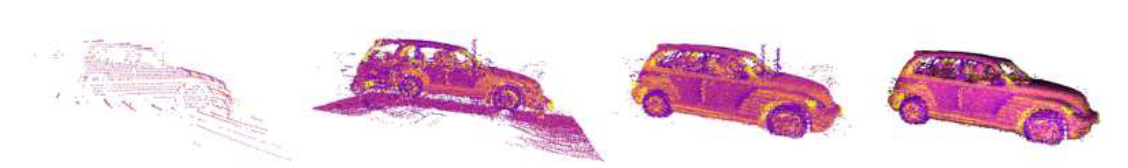
\includegraphics[width=.68\linewidth]{Images/IndividualLidarSweep to surfelmeshing.png}

\vspace{1mm}
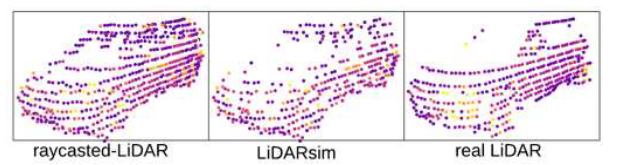
\includegraphics[width=.50\linewidth]{Images/RaycastvsLiDARsimvsRealLiDAR.png}
\caption{Asset reconstruction and sensor modelling in LiDARsim.
Top: an individual sweep, accumulated observations, symmetry completion,
and the refined surfel asset. Bottom: ray-cast measurements, measurements
with learned ray drop, and real LiDAR observations.
Reproduced from Figures~4 and~7 of Manivasagam et al.
\parencite{manivasagamLiDARsimRealisticLiDAR2020}.
The panels illustrate changes in geometry and sampling. Training utility
requires separate evaluation on real data.}
\label{fig:lidarsim-pipeline}
\end{figure}

This approach permits controlled scene composition while retaining
geometric detail from real observations. Its coverage nevertheless depends
on the reconstructed assets, and the demonstrated vehicle reconstruction
does not establish equivalent support for deformable road users
\parencite{manivasagamLiDARsimRealisticLiDAR2020}.
Consequently, realistic individual assets should not be equated with
coverage of all relevant traffic participants or configurations.

\subsection{Learned scans and conditional completion}

Learned scan generation shifts the modelling emphasis from explicit scene
assets to the distribution of sensor observations. LiDARGen represents
range and intensity in \glspl{range-image}, using stochastic denoising to
generate scans and conditional \gls{densification} to complete sparse
inputs. Its KITTI-360 and nuScenes experiments use sensor-specific angular
representations \parencite{zyrianovLearningGenerateRealistic2022}.
This representation captures the organisation of measurements, but does
not itself provide object identities, semantic labels or an editable scene.
Furthermore, completing an existing scan retains information from that
input, whereas unconditional generation samples a new observation.
These capabilities serve different purposes, so evidence for completion
must be distinguished from evidence that generated scans can train a
perception model.

\subsection{Requirements across generation pipelines}

Table~\ref{tab:lidar-generation-comparison} summarises the practical
consequences of these design choices. Scene-based methods provide access
to geometry and annotations, but require suitable observation models.
Learned methods capture scan patterns, while labels and scene control
remain additional requirements. Hybrid methods connect these capabilities
without eliminating dependence on real recordings.

\begin{table}[htbp]
\caption{Comparison of the reviewed LiDAR generation pipelines.
Entries summarise capabilities and constraints, rather than rank
perception performance.}
\label{tab:lidar-generation-comparison}
\small
\begin{tabularx}{\linewidth}{@{}lYY@{}}
\toprule
\textbf{Method} & \textbf{Generation basis} & \textbf{Key requirement or constraint} \\
\midrule
PreSIL \parencite{hurlPreciseSyntheticImage2019}
& Virtual scenes with generated annotations
& Forward-facing scans without reflectance or motion distortion. \\
SynLiDAR \parencite{xiaoTransferLearningSynthetic2022}
& Virtual scenes with semantic labels
& Real data for intensity modelling and class mapping for transfer. \\
LiDARsim \parencite{manivasagamLiDARsimRealisticLiDAR2020}
& Reconstructed assets with learned ray drop
& Real recordings and annotations for asset construction and sensor modelling. \\
LiDARGen \parencite{zyrianovLearningGenerateRealistic2022}
& Learned range and intensity distributions
& Example scans for learning. Semantic labels are not generated by the scan model. \\
\bottomrule
\end{tabularx}
\end{table}

Across these pipelines, scene diversity describes what is observed,
whereas sensor modelling determines how it is sampled. Paired-scenario
experiments identify material response, scanning motion and
traffic-participant geometry as contributors to the \gls{domain-gap}
\parencite{manivasagamZeroDomainGap2023}.
The implication is that scene coverage, sensor behaviour and annotation
consistency must be assessed together. Visual similarity can reveal
sampling differences, as the LiDARsim example illustrates, but cannot
establish whether generated data improves perception on real measurements.
The next section therefore examines how evaluation connects these data
properties to performance on real perception tasks.

\section{Evaluation and real-data transfer}
\label{sec:rq3}
\label{sec:lidar-evaluation}

Evaluation must distinguish similarity between scans from benefits obtained
by training on them. The reviewed studies provide evidence at both levels,
but their different tasks and protocols require separate interpretation.

\subsection{Scan diagnostics and training evidence}

Geometric errors require aligned, corresponding observations, whereas
unpaired generation needs distributional comparisons. LiDARGen uses
\gls{mmd} and \gls{jsd} on bird's-eye-view (\gls{bev}) histograms and
\gls{frd} on RangeNet++ features. On KITTI-360, ProjectedGAN obtains better
MMD, while LiDARGen obtains better FRD and JSD
\parencite{zyrianovLearningGenerateRealistic2022}.
The disagreement shows that conclusions depend on the representation used
for comparison. These metrics diagnose differences but do not establish
which generated dataset provides better training data.

Training protocols provide complementary evidence. PreSIL reports improved
KITTI pedestrian detection after synthetic pretraining and real
\gls{fine-tuning}. However, selecting its best checkpoint on the evaluation
split can produce optimistic results relative to independent final testing
\parencite{hurlPreciseSyntheticImage2019}.
LiDARsim reports a KITTI hard BEV score of 73.7 at \gls{iou}~0.7, compared
with 42.2 for modified CARLA and 80.0 for real training
\parencite{manivasagamLiDARsimRealisticLiDAR2020}.
This narrows the simulation-to-real difference in that setting, but uses
sensor adaptation and a KITTI-labelled object bank. It is consequently
neither evidence of independence from real data nor a full 3D detection result.

SynLiDAR's mixed-training results (Table~\ref{tab:transfer}) show gains of
2.2 and 2.6 percentage points over real-only training. PCT increases those
gains to 4.4 and 5.2 points \parencite{xiaoTransferLearningSynthetic2022}.
Thus, supplementation helps in the reported settings, while the additional
improvement with translation cannot be attributed to sample quantity alone.
LiDARGen instead applies an existing segmenter to densified scans without
retraining, supporting completion utility rather than synthetic-training
gains \parencite{zyrianovLearningGenerateRealistic2022}.

\begin{table}[htbp]
\caption{SynLiDAR mIoU (\%) reported by Xiao et al., Tables~2--3
\parencite{xiaoTransferLearningSynthetic2022}.
All rows use MinkowskiNet. Evaluation uses SemanticKITTI validation
sequence 08 and SemanticPOSS validation sequence 03.}
\label{tab:transfer}
\small
\begin{tabularx}{\linewidth}{@{}Yrr@{}}
\toprule
\textbf{Training data} & \textbf{SemanticKITTI} & \textbf{SemanticPOSS} \\
\midrule
Real only & 60.3 & 50.6 \\
Real + SynLiDAR & 62.5 & 53.2 \\
Real + PCT-translated SynLiDAR & 64.7 & 55.8 \\
\bottomrule
\end{tabularx}
\end{table}

\subsection{Validity and comparison conditions}

Validation supports model selection, while independent real test data
support final performance estimates
\parencite{raschkaModelEvaluationModel2020}.
Westphal and Brannath address selection-induced optimism with a specialised
multiple-testing correction, which does not justify ordinary repeated
test-set tuning \parencite{westphalImprovingModelSelection2019}.
For LiDAR, independence must also extend to generator inputs and
reconstructed assets. Comparisons should document scene splits, sensor
settings, class mappings, training budgets and access to real labels.

Task-appropriate real-data \gls{ap} or \gls{miou}, supported by repeated
runs and class- and range-specific analysis, then provides direct evidence
of training utility. Sensor diagnostics help explain the result.
Evaluation of an already-trained autonomy system is a different objective:
aggregate perception scores need not track planning discrepancies
\parencite{manivasagamZeroDomainGap2023}.
These distinctions determine how broadly the reviewed findings can be interpreted.


\section{Discussion}
\label{sec:discussion}

PreSIL, LiDARsim and SynLiDAR demonstrate benefits under different training
protocols, supporting method selection around a defined task
\parencite{hurlPreciseSyntheticImage2019,manivasagamLiDARsimRealisticLiDAR2020,
xiaoTransferLearningSynthetic2022}.
Scene-based methods provide object and annotation control, learned models
capture scan patterns, and hybrids connect these capabilities. Their
real-data dependencies and output labels must therefore be considered
alongside visual realism when choosing a training pipeline.

\subsection{Coverage and further research}

Average similarity does not establish rare-case coverage. Shumailov et al.
show loss of distribution tails during recursive synthetic-data training
in language, VAE and mixture-model settings
\parencite{shumailovAIModelsCollapse2024}.
This motivates tracking provenance and uncommon scenarios, but does not
establish collapse in one-pass LiDAR augmentation. Scenario-specific real
evaluation remains necessary to substantiate coverage claims.

A useful research direction is to connect sensor diagnostics to training
outcomes. LiDARGen's metric disagreement and paired-scenario analyses do
not establish a general diagnostic-to-utility relationship
\parencite{zyrianovLearningGenerateRealistic2022,manivasagamZeroDomainGap2023}.
Varying ray drop or angular sparsity while fixing scenes, labels, model and
training budget could reveal which changes improve class- and
range-specific performance on independent real data. Broader searching
is required before claiming novelty, and any result would remain qualified
by the sensors and tasks tested.

\subsection{Limitations and implications}

The selected collection, incomplete systematic screening and pending
independent author verification mean that relevant or contradictory work
may be missing. Differences in sensors, tasks and protocols prevent pooling
scores, while incomplete extraction of resource costs and repeated-run
uncertainty prevents reliable efficiency or robustness rankings.
Several studies also report validation outcomes rather than independent
final tests. These limitations constrain generalisation without negating
benefits in the reported experiments. The resulting conclusion is that
synthetic data can provide targeted support when its contribution and
real-data dependencies are explicitly evaluated.

\section{Conclusion}
\label{sec:conclusion}

This review connected general generation approaches to automotive LiDAR
and its evaluation. Simulation, learned generators and hybrids offer
different balances of scene control, coverage and dependence on real data.
Useful training datasets require sensor sampling and annotation consistency
in addition to plausible geometry.

The selected studies support synthetic pretraining and supplementation in
particular perception settings, but do not establish a universal ranking
or replacement for real data. Similarity and completion evaluations provide
complementary evidence, while controlled assessment on independent real
observations most directly establishes training utility. Connecting sensor
diagnostics and scenario coverage to consistent downstream gains could
help identify which aspects of synthesis merit improvement and where real
measurements remain necessary.

\clearpage
\begingroup
\raggedright
\eyebrow{Acknowledgement of AI assistance}
\vspace{2mm}
{\small\color{muted}OpenAI ChatGPT was used to draft and rephrase text, review structure, and help identify candidate academic sources.
	The authors remain responsible for verifying sources, assessing the evidence
	and approving the final text.\par}
\printbibliography[heading=bibintoc,title={References}]
\endgroup
\clearpage
\begingroup
% Compact list spacing keeps the expanded glossary readable without a short final page.
\newglossarystyle{papercompact}{%
  \setglossarystyle{list}%
  \renewcommand*{\glsgroupskip}{}%
  \renewenvironment{theglossary}{\begin{description}%
    \setlength{\itemsep}{2pt}\setlength{\parsep}{0pt}}{\end{description}}%
}
\printnoidxglossary[title={Glossary},style=papercompact]
\endgroup
\clearpage
\appendix
\titleformat{\section}{\Large\bfseries}{\makebox[11mm][l]{\color{muted}\fontsize{11}{13}\selectfont\thesection}}{0pt}{}
% Retained as writing examples, excluded from the research paper by default.
% \section{Mathematical notation examples}
\label{app:mathematics}
\draftnote{Template examples only. Adapt the notation and objectives to the
research methods actually used.}

\subsection{Inline and numbered expressions}
Let $\mathcal{D}_{\mathrm{syn}}=\{(\bm{x}_i,y_i)\}_{i=1}^{n}$ denote a
synthetic training dataset, where $\bm{x}_i\in\mathbb{R}^{d}$ is a feature
vector and $y_i$ its target. An illustrative empirical training objective is
\begin{equation}
  \hat{\theta}=\operatorname*{arg\,min}_{\theta\in\Theta}
  \frac{1}{n}\sum_{i=1}^{n}\ell\bigl(f_{\theta}(\bm{x}_i),y_i\bigr).
  \label{eq:training-objective}
\end{equation}
Here $f_{\theta}$ is the model and $\ell$ is its loss function.
Equation~\eqref{eq:training-objective} demonstrates a clickable equation reference.

\subsection{Aligned expressions}
For regression, a squared-error loss and an illustrative real-data evaluation
risk can be written as
\begin{align}
  \ell(\hat{y},y)&=(\hat{y}-y)^2, \label{eq:squared-loss}\\
  R_{\mathrm{real}}(\theta)&=
  \mathbb{E}_{(\bm{x},y)\sim P_{\mathrm{real}}}
  \!\left[\ell\bigl(f_{\theta}(\bm{x}),y\bigr)\right].
  \label{eq:real-risk}
\end{align}
Training on synthetic data does not, by itself, establish performance on real
data; Equation~\eqref{eq:real-risk} defines a separate evaluation quantity.

\subsection{Matrices and cases}
A feature matrix and a binary decision rule illustrate two other useful forms:
\[
  \bm{X}=\begin{bmatrix}
    x_{11} & \cdots & x_{1d}\\
    \vdots & \ddots & \vdots\\
    x_{n1} & \cdots & x_{nd}
  \end{bmatrix},
  \qquad
  \hat{y}=\begin{cases}
    1, & p_{\theta}(y=1\mid\bm{x})\geq\tfrac{1}{2},\\
    0, & \text{otherwise}.
  \end{cases}
\]

\end{document}

